
\subsubsection{Boundary-klasse: Steering}

\begin{figure}[h]
\centering
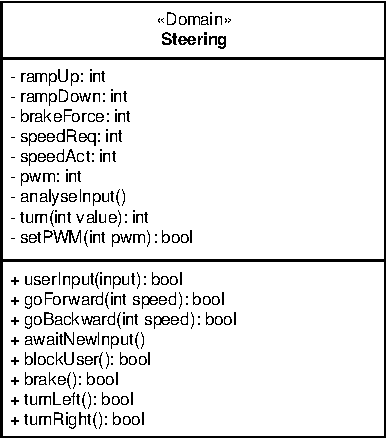
\includegraphics[]{../fig/diagrammer/bil/cd_steering.pdf}
\caption{Klassebeskrivelse af boundary-klassen Sterering}
\label{fig:cd_Sterering}
\end{figure}

\textbf{Attributter}

\begin{table}[H]
\begin{tabularx}{\textwidth}{| Z | Z | L{10cm} |} \hline
Navn & Type & Beskrivelse \\\hline
\texttt{pwm\_} & \texttt{int} &tekst.\\\hline
\texttt{direction\_} & \texttt{bool} &tekst.\\\hline
\texttt{minServoPWM\_} & \texttt{int} &tekst.\\\hline
\texttt{maxServoPWM\_} & \texttt{int} &tekst.\\\hline
\texttt{dataClassPtr\_} & \texttt{Data*} &tekst.\\\hline
\texttt{dState\_} & \texttt{double } &tekst.\\\hline
\texttt{iState\_} & \texttt{double} &tekst.\\\hline
\texttt{iMax\_} & \texttt{double } &tekst.\\\hline
\texttt{iMin\_} & \texttt{double } &tekst.\\\hline
\texttt{iGain\_} & \texttt{double } &tekst.\\\hline
\texttt{pGain\_} & \texttt{double } &tekst.\\\hline
\texttt{dGain\_} & \texttt{double } &tekst.\\\hline
\texttt{error\_} & \texttt{double } &tekst.\\\hline
\texttt{pTemp\_} & \texttt{double } &tekst.\\\hline
\texttt{dTemp\_} & \texttt{double } &tekst.\\\hline
\texttt{iTemp\_} & \texttt{double } &tekst.\\\hline


\end{tabularx}
\caption{Attributter for klassen Steering}
\label{table:attr_steering}
\end{table}

\newpage
\textbf{Metoder} 

%TODO fix position

\begin{table}[H]
\begin{tabularx}{\textwidth}{| L{2.5 cm} | Z |} \hline
Prototype & \texttt{int userInput(unsigned char speedForward, unsigned char speedBackward, 
	char turn, char brake)} \\\hline
Parametre & \texttt{speedForward} \newline Den ønskede hastighed fremad. 0..255\newline
		\texttt{speedBackward} \newline Den ønskede hastighed bagud. 0..255\newline
		\texttt{turn} \newline Den ønskede drejning på forhjul. -127..127\newline
		\texttt{brake} \newline Der skal bremses. 0..1\newline 
 \\\hline
Returværdi &  \texttt{int} \newline 1 hvis alle operationer er gået okay ellers -1. \\\hline
Beskrivelse & Metoden sørger for at opdaterer retning og hastighed på bilen. \\\hline
\end{tabularx}
\caption{Metodebeskrivelse for \texttt{userInput}}
\label{table:met_getdistance}
\end{table}